\documentclass{scrartcl}
\usepackage[utf8]{inputenc}
\usepackage{listings}
\usepackage{geometry}
\usepackage[T1]{fontenc}
\usepackage{appendix}
\usepackage{graphicx}
\usepackage{amsthm}
\usepackage{amssymb}
\usepackage{amsmath}
\usepackage{mathtools}
\usepackage{float}
\usepackage[UKenglish]{babel}
\usepackage{url}
\usepackage{titling}
\usepackage{multirow}
\usepackage{setspace}
\usepackage{subcaption}

\usepackage{algorithm}
\usepackage[noend]{algpseudocode}
\usepackage{amsfonts}

\DeclarePairedDelimiter\ceil{\lceil}{\rceil}
\DeclarePairedDelimiter\floor{\lfloor}{\rfloor}
\DeclareMathOperator{\Tr}{Tr}
\DeclareMathOperator*{\argmin}{\arg\!\min}
\DeclareMathOperator*{\argmax}{\arg\!\max}

\title{Computational Statistics\\Project Report}
%\author{...}

\begin{document}

    \setstretch{1.25}

    \maketitle

    \section{Introduction}
    The Markov Chain Monte Carlo (MCMC) sampling tries to investigate properties of distributions by drawing
    random samples. This is a sequential process, where the drawing of a random sample at any given
    time depends only on its immediate predecessor. In this project a variant of the MCMC algorithm from the paper
    \cite{lau2019} is reimplemented and an attempt is made to reproduce the results of the experiments. The paper under consideration builds on the ideas of
    \cite{metropolis1953,geyer1992,liu2000} and \cite{yang2019}.
    The source code under MIT license for this project can be found in the GitHub repository
    \begin{align*}
        \texttt{github.com/rinkwitz/Adaptive\_Plateau\_MCMC}\,.
    \end{align*}
    Since the simulation of Markov chains is very time-consuming, you can download already simulated MCMC runs under the link
    \begin{align*}
        \texttt{drive.google.com/file/d/1OzUR6-axu2M8hrUERXLregBqmXdpoS-Y/view?usp=sharing}\,.
    \end{align*}

    \section{Adaptive Component-wise Multiple-Try Metropolis Algorithm} The core algorithm
    of the paper \cite{lau2019} consists of a MCMC algorithm which fulfills three properties. First, the algorithm suggests
    several suggestions from different plateau distributions during sampling. This happens independently for all
    components of a sample. Lastly, plateau distributions adapt their shape depending on the frequency of the accepted sample proposals.

	\subsection{Plateau Proposal Distributions}
    The MCMC algorithm in \cite{lau2019} uses \textit{non-overlapping plateau proposal distributions} for sampling.
	The underlying probability density function $f$ is a combination of the density of a uniform distribution
	with exponential decaying tails. Here the density $f$ is constant around a mean value $\mu$ in the closed interval $[\mu-\delta,\mu+\delta]$ with $\delta > 0$.
	Outside this interval the distribution follows an exponential decay with its tail width determined by $\sigma_i > 0$,
	depending on whether you are on the left or right side of the interval $[\mu-\delta,\mu+\delta]$. If you define
	an unnormalized density function
	\begin{align*}
		\tilde{f}(y;\mu,\delta,\sigma_1,\sigma_2)&=\begin{cases}
			\exp\left( -\frac{1}{2\sigma_1^2}[y-(\mu-\delta)]^2 \right)&\quad ,y<\mu-\delta\\
           1&\quad ,\mu-\delta\leq y\leq\mu+\delta\\
           \exp\left( -\frac{1}{2\sigma_2^2}[y-(\mu+\delta)]^2 \right)&\quad ,y>\mu+\delta
		\end{cases}
	\end{align*}
    and then calculate the following integral
    \begin{align*}
        C(\delta,\sigma_1,\sigma_2)&=\int\limits_{-\infty}^\infty\tilde{f}(y;\mu,\delta,\sigma_1,\sigma_2) dy\\
        &= \int\limits_{-\infty}^{\mu-\delta}\exp\left( -\frac{1}{2\sigma_1^2}[y-(\mu-\delta)]^2 \right)dy+
        \int\limits_{\mu-\delta}^{\mu+\delta}1dy+
        \int\limits_{\mu+\delta}^{\infty}\exp\left( -\frac{1}{2\sigma_2^2}[y-(\mu+\delta)]^2 \right)dy\\
        &=\frac{\sqrt{2\pi\sigma_1^2}}{2}+2\delta+\frac{\sqrt{2\pi\sigma_1^2}}{2}
    \end{align*}
    as the sums of 2 half gaussian integrals and one integral over a constant function, then the normalized probability density function is $f(y; \mu,\delta,\sigma_1,\sigma_2)=C(\delta,\sigma_1,\sigma_2)^{-1}\tilde{f}(y;\mu,\delta,\sigma_1,\sigma_2)$ \cite{lau2019}.
    Using $f$ you can define the plateau probability density distributions $T_{j,k}$, $j\in\{1,\dots,M\}$ for the trial proposals of the $k$-th component as
    \begin{align*}
        T_{j,k}(x,y)&=\begin{cases}
                          f(y;x,\delta_1,\sigma,\sigma)&,j=1\\
                          \frac 12 f(y;x-(2j-3)\delta-\delta_1,\delta,\sigma,\sigma)+\frac 12 f(y;x+(2j-3)\delta+\delta_1,\delta,\sigma,\sigma)&,j=2,\dots M-1\\
                          \frac 12 f(y;x-(2M-3)\delta-\delta_1,\delta,\sigma_0,\sigma)+\frac 12 f(y;x+(2M-3)\delta+\delta_1,\delta,\sigma,\sigma_1)&,j=M
        \end{cases}
    \end{align*}
    with values $\delta_1,\delta,\sigma,\sigma_0,\sigma_1>0$. In figure \ref{trial_proposals}
    you can see the trial proposal propability density distributions for the parameters $M=5, \delta_1=\delta=1,\sigma=0.05,\sigma_0=\sigma_1=0.5$. One can see that the
    distributions overlap only at their exponential decaying tails. The outer tails decrease with the larger $\sigma_0, \sigma_1$ values
    shallower than the remaining tails. In the paper \cite{lau2019}, the authors consistently use the values $\delta=\delta_1=2,\sigma=0.05,\sigma_0=\sigma_1=3$.

    \begin{figure}
        \centering
        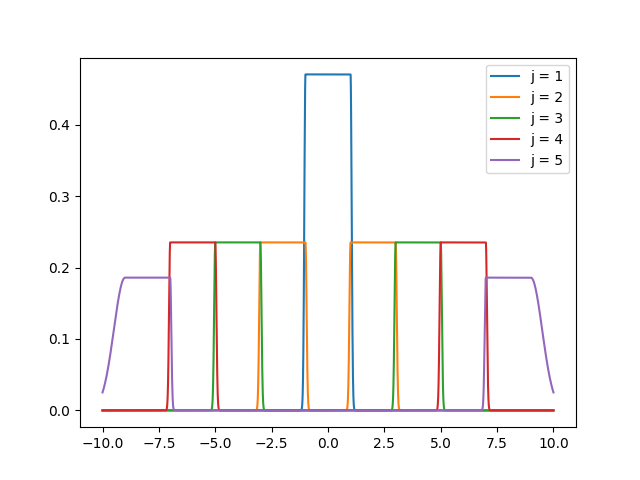
\includegraphics[scale=0.6]{../figs/fig_2b.png}
        \caption{Trial proposal propability density distributions for $M=5$}
        \label{trial_proposals}
    \end{figure}

    \subsection{Component-wise Multiple-Try Metropolis} The component-wise multiple-try Metropolis algorithm \cite[Algorithm 1]{lau2019},
    which forms the basis of the sampling procedure, starts from a starting position
	$x_0\in\mathbb{R}^d$. For each MCMC realization $x_n$ with $n\in\{1,\dots,N\}$ the following procedure is used for each one of the $d$ components. If $x=(x_1,\dots,x_d)$ is the last sampled candidate of the MCMC algorithm, then the algorithm proposes trials $z_j$
    for $i=1,\dots,M$ by sampling it from the distributions $T_{j,k}(x_k,\cdot)$. In my reimplementation
    I use a rejection sampling procedure \cite{rejection_sampling}. For this purpose I use an uniform distribution to generate the samples over the following intervals
%    \begin{itemize}
%        \item $j=1:I_1=[x_k-\delta_1-t_1,x_k+\delta_1+t_1]$ mit $t_1 = \sqrt{-2\sigma^2\log(0.0001C(\delta_1,\sigma,\sigma))}$,
%        \item $j=2,\dots,M-1:I_2=[x_k-2(j+1)\delta-\delta_1-t_2,x-2j\delta-\delta_1+t_2]\cup[x_k+2j\delta+\delta_1-t_2,x+2(j+1)\delta-\delta_1+t_2]$ mit $t_2=\sqrt{-2\sigma^2\log(0.0002C(\delta,\sigma,\sigma))}$, und
%        \item $j=M:I_3=[x_k-2(M+1)\delta-\delta_1-t_{32},x_k-2M\delta-\delta_1+t_{31}]\cup[x_k+2M\delta+\delta_1-t_{31},x_k+2(M+1)\delta+\delta_1+t_{32}]$ mit $t_{31}=\sqrt{-2\sigma^2\log(0.0002C(\delta,\sigma,\sigma_0))},t_{32}=\sqrt{-2\sigma_0^2\log(0.0002C(\delta,\sigma,\sigma_0))}$.
%    \end{itemize}
    \begin{align*}
        I_j = \begin{cases}
                  [x_k-\delta_1-t_1,x_k+\delta_1+t_1]\\\text{ for }j=1\text{ with }t_1 = \sqrt{-2\sigma^2\log(0.0001C(\delta_1,\sigma,\sigma))},\vspace{.25cm}\\
                  [x_k-2(j+1)\delta-\delta_1-t_2,x-2j\delta-\delta_1+t_2]\cup[x_k+2j\delta+\delta_1-t_2,x+2(j+1)\delta-\delta_1+t_2]\\\text{ for }j=2,\dots,M-1\text{ with }t_2=\sqrt{-2\sigma^2\log(0.0002C(\delta,\sigma,\sigma))},\text{ or}\vspace{.25cm}\\
                  [x_k-2(M+1)\delta-\delta_1-t_{32},x_k-2M\delta-\delta_1+t_{31}]\cup[x_k+2M\delta+\delta_1-t_{31},x_k+2(M+1)\delta+\delta_1+t_{32}]\\\text{ for }j=M\text{ with }t_{31}=\sqrt{-2\sigma^2\log(0.0002C(\delta,\sigma,\sigma_0))},t_{32}=\sqrt{-2\sigma_0^2\log(0.0002C(\delta,\sigma,\sigma_0))}.
        \end{cases}
    \end{align*}
    These intervals enable effective sampling in the range of $T_{j,k}(x_k,\cdot)$ where the probability density function is greater than $0.0001$.
    To do this, one samples a $u\sim U(0,1)$ and a $y\sim U(I_i)$ until
    \begin{align*}
        u < \frac{T_{j,k}(x_k,y)}{c|I_i|}
    \end{align*}
    is fulfilled where $|I_j|$ is the width of the used interval $I_j$, $g_j$ is the probability density function of the uniform distribution over $I_j$ and $c_j$ has the following values situation dependent
    \begin{itemize}
        \item $j=1:\quad c_1=\sup\limits_{y\in I_1}\frac{T_{1,k}(x_k,y)}{g_1(y)}=\frac{|I_1|}{C(\delta_1,\sigma,\sigma)}$,
        \item $j=2:\quad c_j=\sup\limits_{y\in I_j}\frac{T_{j,k}(x_k,y)}{g_j(y)}=\frac{|I_j|}{2C(\delta,\sigma,\sigma)}$, and
        \item $j=M:\quad c_M=\sup\limits_{y\in I_M}\frac{T_{M,k}(x_k,y)}{g_M(y)}=\frac{|I_M|}{2C(\delta,\sigma,\sigma_0)}$.
    \end{itemize}
    Afterwards the weights associated with the trials are
    \begin{align*}
        w_{j,k}&=\pi((z_j;x_{[-k]}))T_{j,k}(x_k,z_j)\lambda_{j,k}(x_k,z_j),\quad\text{for }j=1,\dots,M
    \end{align*}
    are calculated whereby $(z;x_{[-i]})\in\mathbb{R}^d$ denotes the vector, which is identical to $x$ in all entries except the $i$-th one where it takes on the value $z$.
    In addition, the non-negative and symmetric function
    \begin{align*}
        \lambda_{j,k}(x,y)&=|y-x|^{2.5}%T_{j,k}(x,y)
    \end{align*}
    is used. Here the authors of \cite{lau2019} refer to the results of \cite{yang2019}. Thus, suggestions $(z_j;x_{[-k]})$ have a high weight, which have a high probability with regard to
    the target distribution $\pi$, whose new proposal $z_j$ for the $k$-th component regarding $T_{j,k}(x_k,\cdot)$ is very likely and where the distance function $\lambda_{j,k}$ is far enough away from $x_k$.
    Proportionally to the weights $w_{1,k},\dots,w_{M,k}$ a $y\in\{z_1,\dots,z_M\}$ is then randomly drawn and for $j=1,\dots,M-1$ the algorithm samples
    $x_j^*\sim T_{j,k}(y,\cdot)$. Finally one calculates
    \begin{align*}
        \alpha&=\min\left\{ 1,\frac{w_{1,k}(z_1,x)+\dots+w_{M,k}(z_M,x)}{w_{1,k}(x_1^*,(y;x_{[-k]}))+\dots+w_{M-1,k}(x_{M-1}^*,(y;x_{[-k]}))+w_{M,k}(x_k,(y;x_{[-k]}))} \right\}
    \end{align*}
    and with that probability $\alpha$ the algorithm accepts the new proposal and sets $x_n=(y;x_{[-k]})$. Otherwise the algorithm keeps the old proposal and sets $x_n=x$.

    \subsection{Adaption of Proposal Distributions}
    In \cite{lau2019} it is proposed to adapt the widths $\delta$ and $\delta_0$ of the plateau distributions.
    In my implementation every $L$ iterations it measures how high the number of selected suggestions $c_{j,k}$ from the plateau distributions $T_{j,k}$ are in this interval.
    If the middle plateau distribution is called much more than the average, that is $c_{j,k}>L\eta_1$ with $\eta_1\in(0,1)$, then
    the algorithm assumes that the plateaus are too wide and halves $\delta$ and $\delta_1$ accordingly for
    the following iterations. If, on the other hand, the outermost plateau distributions are selected much more than the average, in especially
    $c_{M,k}>\eta_2L$ with $\eta_2\in(0,1)$, then the algorithm assumes that the plateaus are too small and doubles
    $\delta$ and $\delta_1$. The adaptations only take place with a constantly decreasing probability of $\max(0.99^{n-1},1/\sqrt{n})$. This implementation of the adaptation procedure is based on \cite[Algorithm 2]{lau2019}.

    \section{Experiments and Results}

    \subsection{Performance Measures}
    \subsubsection{Integrated Autocorrelation Times}
    The authors in the paper \cite{lau2019} use two performance measures to assess the effectiveness of the implemented
    algorithm. One of these is the integrated autocorrelation times (ACT), which is measured in $R$ MCMC
    simulations with $N$ steps for $K$ components. Let in the following be
    $X_t^{(r)}=(X_{t,1}^{(r)},\dots,X_{t,K}^{(r)})$ the result of the $r$-th MCMC simulation at step $t$, where
    $r\in\{1,\dots,R\}$ and $t\in\{1,\dots,N\}$. First of all, one estimates the normalized autocorrelation $\hat{p}_{\tau,k}^{(r)}$
    by means of
    \begin{align*}
        \hat{c}_{\tau,k}^{(r)}&=\frac{1}{N-\tau}\sum\limits_{i=1}^{N-\tau}(X_{i,k}^{(r)}-\bar{X_k}^{(r)})(X_{i+\tau,k}^{(r)}-\bar{X_k}^{(r)})\text{ and}\\\
        \hat{p}_{\tau,k}^{(r)}&=\frac{\hat{c}_{\tau,k}^{(r)}}{\hat{c}_{0,k}^{(r)}}
    \end{align*}
    where $\bar{X_k}^{(r)}=1/N\sum\nolimits_{i=1}^NX_{i,k}^{(r)}$ is the arithmetic mean of the $k$-th component in the $r$-th
    simulation. Afterwards one approximates the integrated autocorrelation times as
    \begin{align*}
        \hat{\tau}_{k}^{(r)}&=1+2\sum\limits_{\tau=1}^M\hat{p}_{\tau,k}^{(r)}
    \end{align*}
    \cite{autocorrelation_blog} where $M\ll N$. To determine $M$ the implementation uses a \textit{initial monotone sequence estimator}
    as introduced by \cite [geyer1992]. where $M$ is the largest natural number, so that $\hat{p}_{\tau,k}^{(r)} > 0$ applies to all $\tau\in\{1,\dots,2M+1\}$ and
    and the subsequence $(\hat{p}_{2\tau,k}^{(r)} + \hat{p}_{2\tau+1,k}^{(r)})_{\tau=1,\dots,M}$ is monotone \cite{geyer1992}.

    \subsubsection{Average Squared Jump Distance}
    Another performance measure is the average squared jump distance (ASJD)
    \begin{align*}
        \text{ASDJ}_k^{(r)}=\frac{1}{N}\sum\limits_{i=1}^N|X_{i,k}^{(r)}-X_{i-1,k}^{(r)}|^2
    \end{align*}
    for the $k$-th component and the $r$-th repetition of the Markov chain \cite{lau2019}.
    Larger ASJD values are preferred, as they indicate that the state-space is better explored \cite{lau2019}.

    \subsection{Experiments}
    \subsubsection{Target Distributions}
    As experiments to test the performance of the adaptive plateau-based MCMC method \cite{lau2019} examines four target distributions
    with the Markov chain. The target distributions are
    \begin{itemize}
        \item $\pi_1:$ a mixture of 4-dimensional Gaussians $\frac12\mathcal{N}(\mu_1,\Sigma_1)+\frac12\mathcal{N}(\mu_2,\Sigma_2)$ with $\mu_1=(5,5,0,0)^T,\mu_2=(15,15,0,0)^T,\Sigma_1=\text{diag}(6. 25,6.25,6.25,0.01),\Sigma_2=\text{diag}(6.25,6.25,0.25,0.01)$,
        \item $\pi_2:$ an 8-dimensional banana distribution with density $f\circ\phi$, where $f$ is the density of an 8-dimensional normal distribution $\mathcal{N}(0,\Sigma_3)$ with $\Sigma_3=\text{diag}(100,1,\dots,1)$ and $\phi(x)=(x_1,x_2+0. 03x_1^2-3,x_3,\dots,x_8)$ for $x\in\mathbb{R}^8$,
        \item $\pi_3:$ a perturbed 2-dimensional gaussian with unnormalized probability density $\tilde{\pi_3}(x)=\exp\left( -x^TAx-\cos\left( \frac{x_1}{0.1} \right) -0.5\cos\left( \frac{x_2}{0.1} \right) \right)$ for $x\in\mathbb{R}^2$ with
        $A=\begin{pmatrix}
                    1 & 1\\
                    1 & 3/2
        \end{pmatrix}$, and
        \item $\pi_4:$ a 1-dimensional bi-stable distribution with unnormalized distribution $\tilde{\pi_4}(x)=\exp\left( -x^4+5x^2-\cos\left( \frac{x}{0.02} \right) \right)$ for $x\in\mathbb{R}$.
    \end{itemize}
    These distributions are shown in Figure \ref{target_distributions}, which is based on \cite[Figure 3]{lau2019}. The representation
    of $\pi_2$ in Figure \ref{target_distributions_pi_2} results from a dimensionally reduced simplification, since a marginal with 6 integration variables was computationally too expensive. One can also recognize this by the fact that the probability density here is greater than that in \cite{lau2019}.
    \begin{figure}
        \centering
        \begin{subfigure}{.45\textwidth}
              \centering
              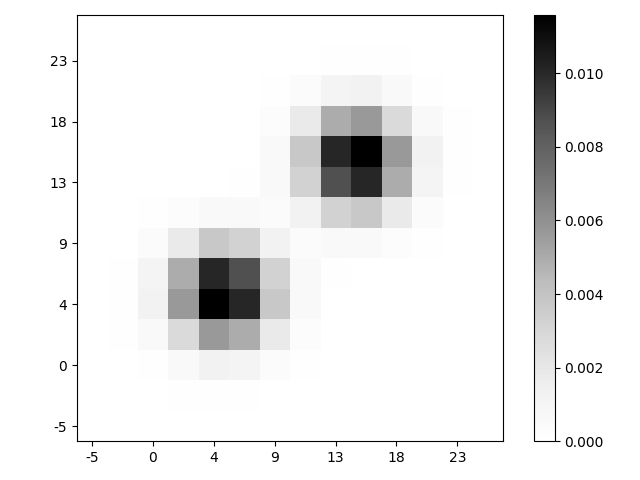
\includegraphics[width=.8\linewidth]{../figs/fig_3_pi_1.png}
              \caption{Joint PDF of components 1 and 2 of $\pi_1$}
              \label{target_distributions_pi_1}
        \end{subfigure}
        \begin{subfigure}{.45\textwidth}
              \centering
              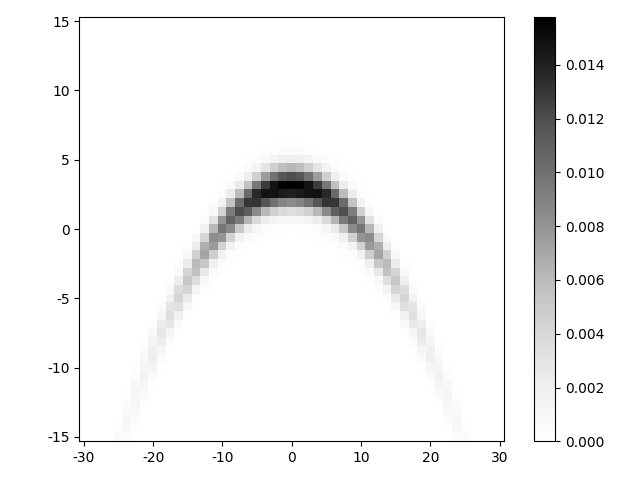
\includegraphics[width=.8\linewidth]{../figs/fig_3_pi_2.png}
              \caption{Joint PDF of components 1 and 2 of $\pi_2$}
              \label{target_distributions_pi_2}
        \end{subfigure}
        \begin{subfigure}{.45\textwidth}
              \centering
              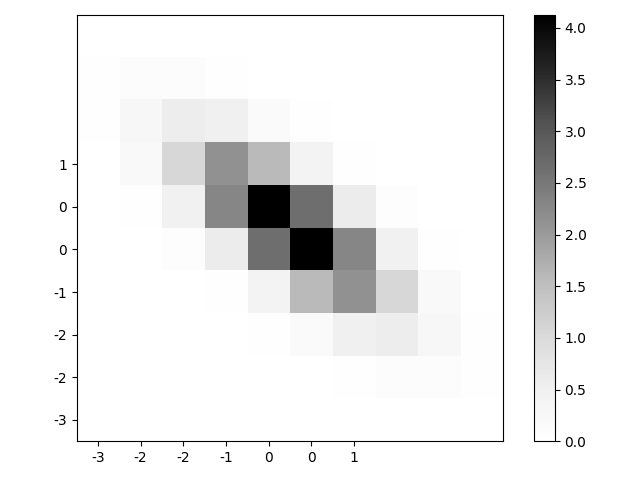
\includegraphics[width=.8\linewidth]{../figs/fig_3_pi_3.png}
              \caption{PDF of $\pi_3$}
              \label{target_distributions_pi_3}
        \end{subfigure}
        \begin{subfigure}{.45\textwidth}
              \centering
              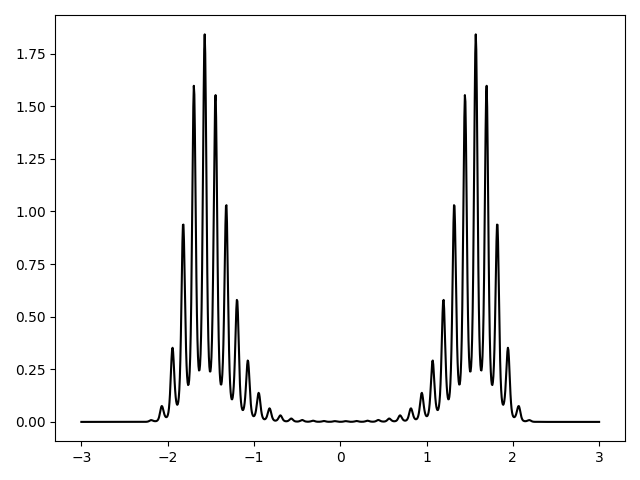
\includegraphics[width=.8\linewidth]{../figs/fig_3_pi_4.png}
              \caption{PDF of $\pi_4$}
              \label{target_distributions_pi_4}
        \end{subfigure}
        \caption{Overview of target distributions}
        \label{target_distributions}
    \end{figure}

    \subsubsection{Simulation Parameter Settings}
    For each of the 4 target distributions $R=200$ MCMC simulations are performed with $N=4000$ iterations for $\pi_1$, $N=10000$ iterations for $\pi_2$, and $N=3000$ iterations for $\pi_3$ and $\pi_4$.
    The remaining parameters are the same for all simulations. These are
    \begin{itemize}
        \item $M=5$ different plateau proposal distributions,
        \item $\delta=\delta_1=2$ widths of plateaus,
        \item $\sigma=0.05$ and $\sigma_0=\sigma_1=3$ flatness of the plateau tails,
        \item $\eta_1=\eta_2=0.4$ minimum amount for an adaptation to occur,
        \item $L=40$ length of the interval between adaptations, and
        \item a burn-in portion of $0.5$ of all iterations.
    \end{itemize}
    These parameters are set exactly as in \cite{lau2019} except $L$, for which there is no exact specification.

    \subsection{Results}
    The violin plots belonging to the experiments can be found for the target distributions $\pi_1$, $\pi_2$, $\pi_3$ and $\pi_4$
    in the figures \ref{violin_plots_pi_1}, \ref{violin_plots_pi_2}, \ref{violin_plots_pi_3} and \ref{violin_plots_pi_4}. One finds the component-wise representation of the ACT distribution in the subfigures \ref{violin_plots_pi_1_act}, \ref{violin_plots_pi_2_act}, \ref{violin_plots_pi_3_act} and \ref{violin_plots_pi_1_act}, and
    the component-wise representation of the ASJD distribution in the subfigures \ref{violin_plots_pi_1_asjd}, \ref{violin_plots_pi_2_asjd}, \ref{violin_plots_pi_3_asjd} and \ref{violin_plots_pi_4_asjd}.
    In order to better estimate the results, the tables \ref{stat_results_act}, \ref{stat_results_log_act} and \ref{stat_results_asjd} contain the median, mean, minimum and maximum in rounded form
    listed for ACT, log-ACT and ASJD results of the experiments.

    \begin{figure}[H]
        \begin{table}[H]
            \centering
            \begin{tabular}{|l|l|l|l|l|l|l|l|l|l|l|l|l|l|l|}
                \hline & $\pi_1$ & $\pi_2$ \\ \hline
                median & 8.999, 9.149, 5.126, 12.131 & 82.767, 88.027, 3.179, 3.17, 3.173, 3.168, 3.17, 3.181 \\\hline
                mean & 9.117, 9.171, 5.019, 14.828 & 92.596, 102.911, 3.168, 3.159, 3.164, 3.156, 3.165, 3.167 \\\hline
                min & 7.594, 7.277, 3.247, 3.042 & 54.33, 46.736, 3.022, 3.007, 3.019, 3.034, 3.032, 3.03 \\\hline
                max & 11.145, 11.295, 6.262, 102.043 & 231.547, 246.187, 3.354, 3.318, 3.325, 3.323, 3.347, 3.354 \\\hline
                \hline & $\pi_3$ & $\pi_4$ \\ \hline
                median & 7.769, 8.155 & 3.62 \\\hline
                mean & 7.821, 8.288 & 3.635 \\\hline
                min & 6.569, 6.84 & 3.337 \\\hline
                max & 9.722, 10.042 & 4.36 \\\hline
            \end{tabular}
            \caption{Rounded statistical results of ACT component-wise}
            \label{stat_results_act}
        \end{table}
    \end{figure}

    \begin{figure}[H]
        \begin{table}[H]
            \centering
            \begin{tabular}{|l|l|l|l|l|l|l|l|l|l|l|l|l|l|l|}
                \hline & $\pi_1$ & $\pi_2$ \\ \hline
                median & 2.197, 2.214, 1.634, 2.496 & 4.416, 4.478, 1.157, 1.154, 1.155, 1.153, 1.154, 1.157 \\\hline
                mean & 2.207, 2.213, 1.605, 2.382 & 4.488, 4.551, 1.153, 1.15, 1.152, 1.149, 1.152, 1.152 \\\hline
                min & 2.027, 1.985, 1.178, 1.113 & 3.995, 3.845, 1.106, 1.101, 1.105, 1.11, 1.109, 1.108 \\\hline
                max & 2.411, 2.424, 1.835, 4.625 & 5.445, 5.506, 1.21, 1.199, 1.202, 1.201, 1.208, 1.21 \\\hline
                \hline & $\pi_3$ & $\pi_4$ \\ \hline
                median & 2.05, 2.099 & 1.286 \\\hline
                mean & 2.053, 2.111 & 1.289 \\\hline
                min & 1.882, 1.923 & 1.205 \\\hline
                max & 2.274, 2.307 & 1.473 \\\hline
            \end{tabular}
            \caption{Rounded statistical results of log-ACT component-wise}
            \label{stat_results_log_act}
        \end{table}
    \end{figure}

    \begin{figure}[H]
        \begin{table}[H]
            \centering
            \begin{tabular}{|l|l|l|l|l|l|l|l|l|l|l|l|l|l|l|}
                \hline & $\pi_1$ & $\pi_2$ \\ \hline
                median & 26.172, 26.186, 5.691, 0.032 & 9.508, 2.907, 2.948, 2.945, 2.942, 2.938, 2.953, 2.952 \\\hline
                mean & 26.191, 26.169, 6.158, 0.041 & 9.791, 2.922, 2.972, 2.965, 2.949, 2.96, 3.033, 2.977 \\\hline
                min & 24.792, 24.357, 5.095, 0.029 & 8.315, 2.837, 2.852, 2.858, 2.854, 2.841, 2.863, 2.86 \\\hline
                max & 27.612, 28.239, 12.865, 0.478 & 21.963, 3.306, 3.698, 3.522, 3.161, 3.534, 3.651, 3.648 \\\hline
                \hline & $\pi_3$ & $\pi_4$ \\ \hline
                median & 1.641, 0.894 & 3.527 \\\hline
                mean & 1.65, 0.905 & 3.514 \\\hline
                min & 1.512, 0.856 & 2.641 \\\hline
                max & 1.779, 1.166 & 3.736 \\\hline
            \end{tabular}
            \caption{Rounded statistical results of ASJD component-wise}
            \label{stat_results_asjd}
        \end{table}
    \end{figure}

    \begin{figure}
        \centering
        \begin{subfigure}{0.42\textheight}
              \centering
              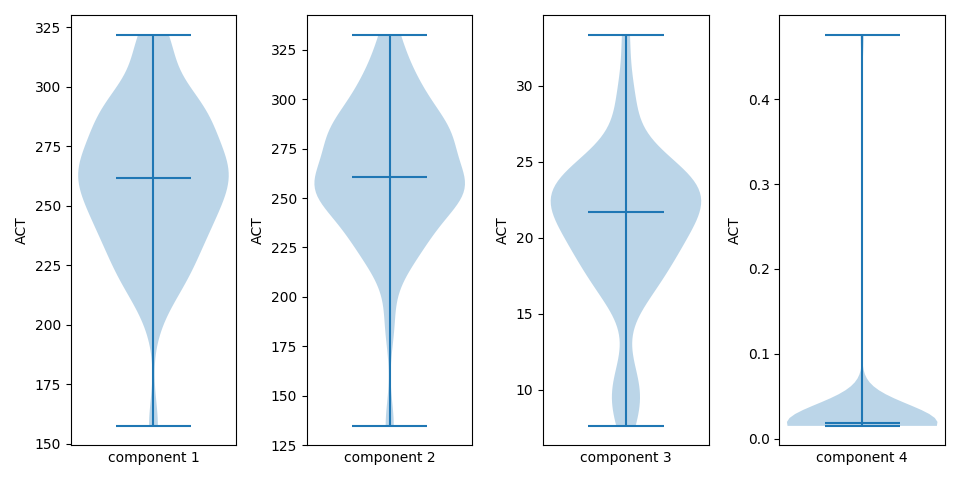
\includegraphics[width=.8\linewidth]{../figs/ACT_pi_1.png}
              \caption{Component-wise ACT distributions for target distribution $\pi_1$}
              \label{violin_plots_pi_1_act}
        \end{subfigure}
        \begin{subfigure}{0.42\textheight}
              \centering
              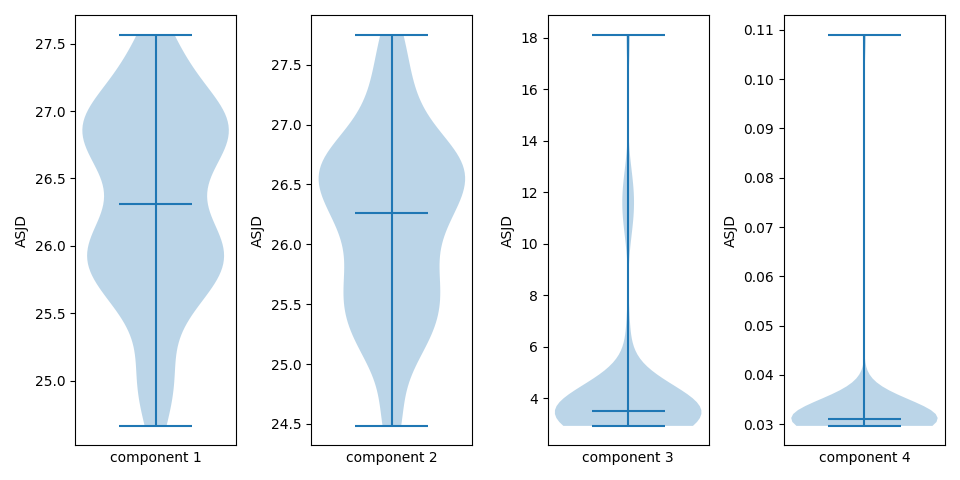
\includegraphics[width=.8\linewidth]{../figs/ASJD_pi_1.png}
              \caption{Component-wise ASJD distributions for target distribution $\pi_1$}
              \label{violin_plots_pi_1_asjd}
        \end{subfigure}
        \caption{Violin plots of performance measures for target distribution $\pi_1$}
        \label{violin_plots_pi_1}
    \end{figure}

    \begin{figure}
        \centering
        \begin{subfigure}{0.42\textheight}
              \centering
              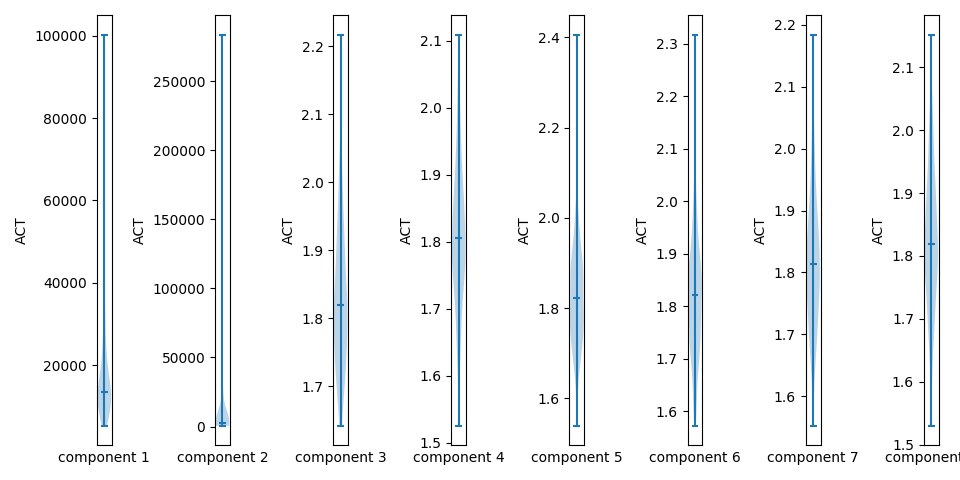
\includegraphics[width=.8\linewidth]{../figs/ACT_pi_2.png}
              \caption{Component-wise ACT distributions for target distribution $\pi_2$}
              \label{violin_plots_pi_2_act}
        \end{subfigure}
        \begin{subfigure}{0.42\textheight}
              \centering
              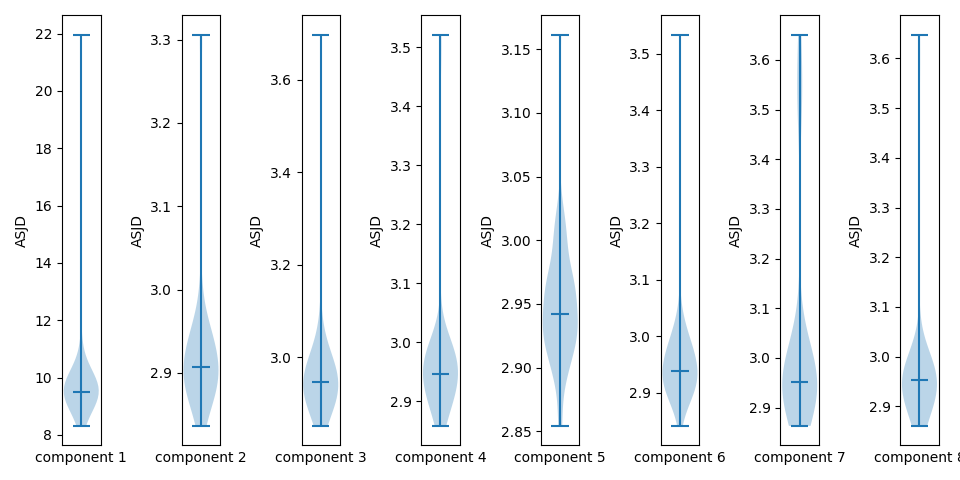
\includegraphics[width=.8\linewidth]{../figs/ASJD_pi_2.png}
              \caption{Component-wise ASJD distributions for target distribution $\pi_2$}
              \label{violin_plots_pi_2_asjd}
        \end{subfigure}
        \caption{Violin plots of performance measures for target distribution $\pi_2$}
        \label{violin_plots_pi_2}
    \end{figure}

    \begin{figure}
        \centering
        \begin{subfigure}{0.42\textheight}
              \centering
              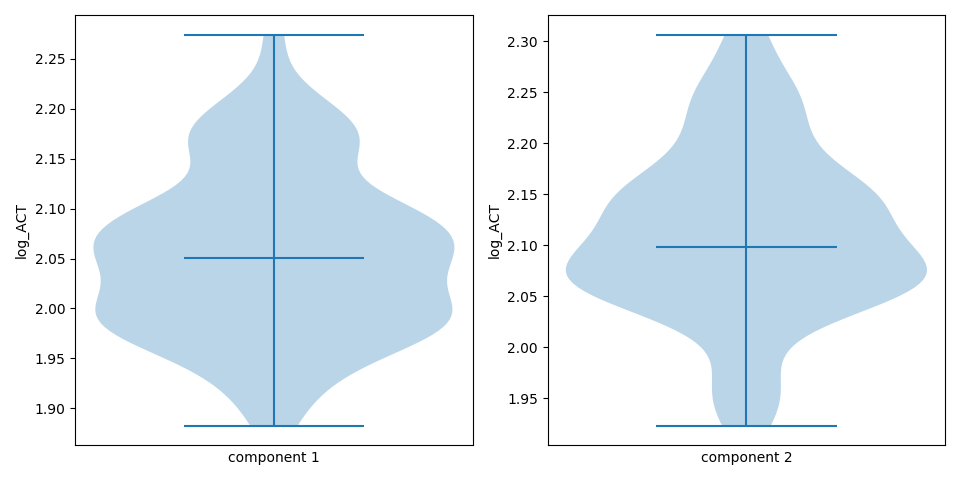
\includegraphics[width=.8\linewidth]{../figs/log_ACT_pi_3.png}
              \caption{Component-wise ACT distributions for target distribution $\pi_3$}
              \label{violin_plots_pi_3_act}
        \end{subfigure}
        \begin{subfigure}{0.42\textheight}
              \centering
              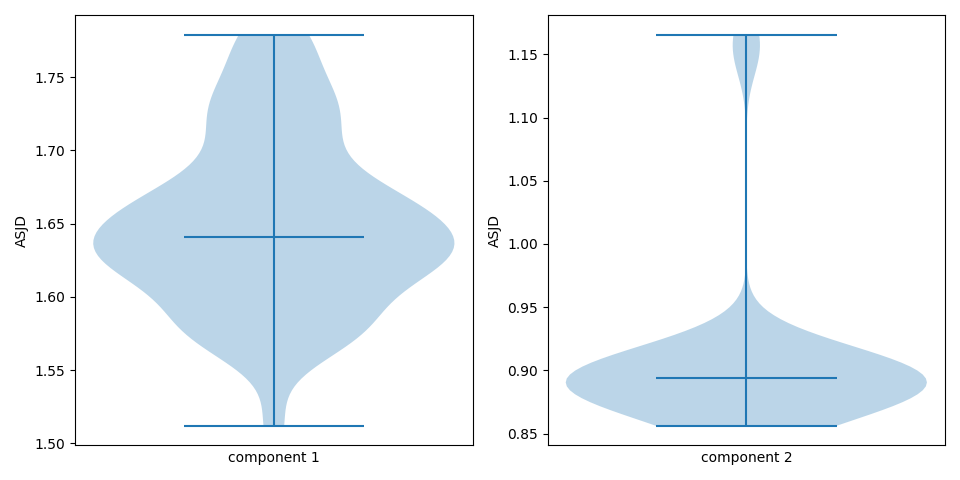
\includegraphics[width=.8\linewidth]{../figs/ASJD_pi_3.png}
              \caption{Component-wise ASJD distributions for target distribution $\pi_3$}
              \label{violin_plots_pi_3_asjd}
        \end{subfigure}
        \caption{Violin plots of performance measures for target distribution $\pi_3$}
        \label{violin_plots_pi_3}
    \end{figure}

    \begin{figure}
        \centering
        \begin{subfigure}{0.42\textheight}
              \centering
              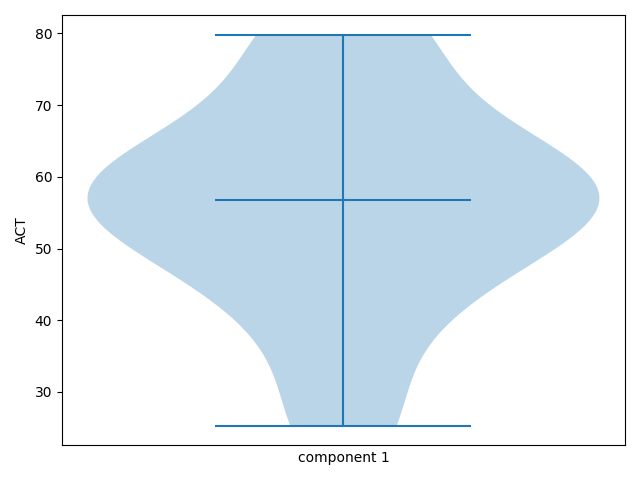
\includegraphics[width=.8\linewidth]{../figs/ACT_pi_4.png}
              \caption{ACT distribution for target distribution $\pi_4$}
              \label{violin_plots_pi_4_act}
        \end{subfigure}
        \begin{subfigure}{0.42\textheight}
              \centering
              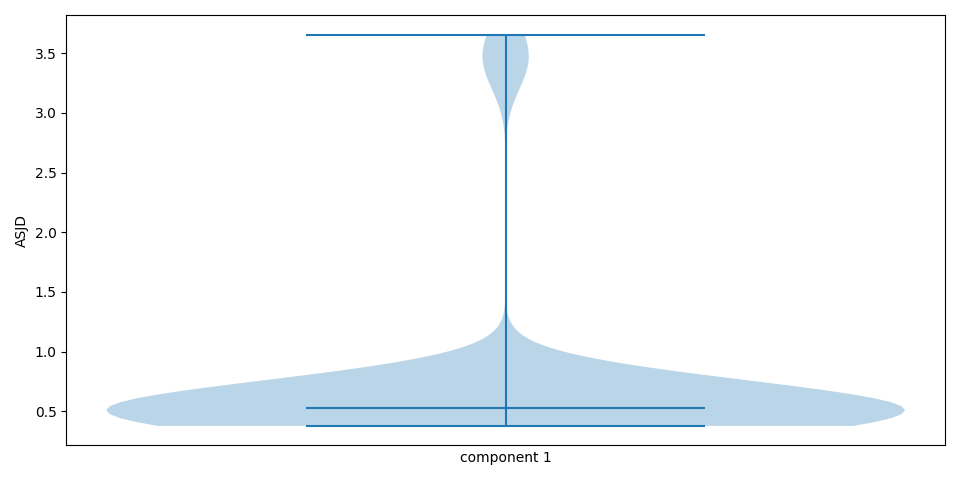
\includegraphics[width=.8\linewidth]{../figs/ASJD_pi_4.png}
              \caption{ASJD distribution for target distribution $\pi_4$}
              \label{violin_plots_pi_4_asjd}
        \end{subfigure}
        \caption{Violin plots of performance measures for target distribution $\pi_4$}
        \label{violin_plots_pi_4}
    \end{figure}

    \section{Discussion}
    The results partly differ significantly from those of the simulations in \cite{lau2019}.
    However, the ratios of the order of magnitude between the components of the ACT and ASJD values appear to be largely consistent.
    In the ACT distributions, there is a close similarity between \cite{lau2019} and this reimplementation (tables \ref{stat_results_act, stat_results_log_act}) in the target distributions
    $\pi_2$ and $\pi_4$, but large deviations for $\pi_1$ and $\pi_3$. There is also a high similarity in the ASJD distributions for the target distributions $\pi_2$ and $\pi_4$
    between \cite{lau2019} and this project (Table \ref{stat_results_asjd}). For the target distributions $\pi_1$ and $\pi_3$ we can observe
    differences in the values, but the ratios between the components are very similar to the ones in \cite{lau2019}.
    Additionally I had the subjective impression that there were big variances in the ACT and ASJD distributions in experiments for the target distribution $\pi_4$.
    Unfortunately I could not compare to the MCMC algorithms MH, AG1 and AG2 \cite{lau2019} due to time constraints. Therefore
    the higher effectiveness of the adaptive plateau-based multiple-try MCMC algorithm, which the authors have concluded in \cite{lau2019},
    can I neither confirm nor dispute.


    \section{Technical Details of Implementation}
    The reimplementation of \cite{lau2019} is written in Python 3 and uses the packages \texttt{Numpy}, \texttt{Scipy}
    and \texttt{Matplotlib}. The four simulations for reproducing the MCMC results can be started with the script
    \texttt{run\_simulations.py}, which runs all four simulations in parallel using \texttt{multiprocessing}.
    The adjustable parameters can be found under \texttt{adjustable parameters} in the script. They follow the naming convention from this report
    and the paper \cite{lau2019}. After the simulations have been run, the script \texttt{create\_violin\_plots.py} can be used to create the
    the violin plots for the results. Furthermore there are two scripts \texttt{create\_fig\_2b.py}
    and \texttt{create\_fig\_3.py} with which reproductions of the Figures 2b and 3 from \cite{lau2019} can be produced.
    If you want to use the MCMC runs already provided in the cloud, one has to copy the extracted \texttt{Numpy}-arrays into the folder
    \texttt{simulations}.

    \bibliographystyle{apalike}
    \bibliography{ref}
\end{document}
